%------------------------------------------------------
%Author             : Daniel Schembri, Jonathan Schwarz
%University         : Pforzheim University
%Date of last edit  : Wed, 03 Sep 2014 14:12:16 +0200
%Filename           : multithreading_with_posix_pthreads.tex
%------------------------------------------------------

\documentclass[10pt,a4paper,DIV=11]{scrreprt}

%British English
\usepackage[UKenglish]{babel}
%utf8
\usepackage[utf8]{inputenc}

%pseudo-code
\usepackage[boxruled,vlined]{algorithm2e}

%for source code listings
\usepackage{listings}

\usepackage[table]{xcolor}

%tikz
\usepackage{tikz}
\usetikzlibrary{arrows,positioning,fit}

%plots
\usepackage{pgfplots}

%blocks - used by tikz-uml, included before
\pgfdeclarelayer{background}
\pgfdeclarelayer{foreground}
\pgfsetlayers{background,main,foreground}

%<,> in tikz-uml
\usepackage[T1]{fontenc}
\usepackage{tikz-uml}

%subfigure
\usepackage{graphicx}
\usepackage{subfigure}

%prevent figure from floating pictures
\usepackage{float}

%footer & header
\usepackage{fancyhdr}

%push footer down
\usepackage[bottom]{footmisc}

%footer & header
\pagestyle{fancy}
%clean footer & header
\fancyhf{}

%bibtex
\usepackage[square,numbers]{natbib}
\usepackage{gensymb}

%equation
\usepackage[tbtags]{amsmath}
\usepackage{amssymb} 

%table of contents with hyperlinks
%always include as last package
\usepackage{hyperref}

%===========================TITLE PAGE=======================================

%university logo
\titlehead
{
    
\includegraphics[width=0.20\textwidth]{files/hspflogo.pdf}\\

    Pforzheim University\\
    School of Engineering\\
}

\subject{Project work}
	
\title
{
    Evolving neutral networks\\
}

\author
{
    by \textbf{Daniel Schembri} - matriculation number: 310026 \\
    and \textbf{Jonathan Schwarz} - matriculation number: 304728
}
\date
{
    Winter term 2013/2014
}
%\today{}}

\publishers
{
    Examiner: Prof Dr Richard Alznauer\\
    Supervisor: Dr Christoph Ussfeller
}


%=========================================GLOBAL SETTINGS=========================================

%footer &header

%\fancyfoot[L]{\textbf{Multi-Threading mit POSIX-pThreads}}
\fancyhead[R]{Page \thepage}
%\fancyhead[L]{\thechapter}

%chapter number and title
\fancyhead[L]{\nouppercase{\leftmark}}
%line
%\renewcommand{\footrulewidth}{0.5 pt}
\usepackage{lmodern}
\addtokomafont{sectioning}{\rmfamily}
\setlength{\parindent}{0mm}

%colour definitions
\definecolor{dkgreen}{rgb}{0,0.6,0}
\definecolor{gray}{rgb}{0.7,0.7,0.7}
%medium gray
\definecolor{mgray}{gray}{0.80}
%light gray
\definecolor{lgray}{gray}{0.97}

%hyperlink settings
%frame around hyperlinks
\hypersetup
{
    colorlinks = false,
    linkcolor = black,
    hypertexnames = false,
    citecolor = green
}

%listing settings
\lstset
{ 
    language=C,                
    basicstyle=\footnotesize\ttfamily,           
    numbers=left,
    stepnumber=5,    
    firstnumber=1,
    numberfirstline=true                 
    numberstyle=\color{black},                 
    numbersep=5pt,                 
    backgroundcolor=\color{white},      
    showspaces=false,             
    showstringspaces=false,         
    showtabs=false,                
    frame=single,                   
    rulecolor=\color{black},       
    tabsize=2,                     
    captionpos=b,                   
    breaklines=true,                
    breakatwhitespace=false,       
    title=\lstname,                    
    keywordstyle=\color{blue},          
    commentstyle=\color{dkgreen}, 
    identifierstyle=\color{black},      
    stringstyle=\color{purple},      
    escapeinside={\%*}{*)},      
    morekeywords={*,...},            
    deletekeywords={...}             
}

\setcounter{tocdepth}{4}  %a deeper contentsmenue
%=====================================DOCUMENT START=========================
\begin{document}

\tikzstyle{line}=[draw]
\tikzstyle{arrow}=[draw, -latex] 

%\renewcommand*\contentsname{Content}
%\renewcommand*\listtablename{Tables}
%\renewcommand*\listfigurename{Figures}
%\renewcommand*\bibname{Literature references}

\maketitle
\thispagestyle{empty}
\newpage
{\large\tableofcontents}
\newpage

\chapter{Artifical neural networks}
\section{Biological and mathematical neurons}
The wish to build reproduce human intelligence has been around since the dawn of mankind. In the effort of building truely intelligent systems, thinking about our brain has turned out to be very useful, helping scientists to extent the scope of technical ideas. One of the basic findings of neuron science is a hypohesis, which suggesst that mental acivity consists primarily of electrochemical acivity in large networks of brain cells, or neurons. Hence the name called neuronal networks. \marginpar{\textit{The biological neuron}}
Although their is still not fully understood, we do know that neurons receive input from other neurons and create an output themselves, as soon as the neuron is activated \textit{it fires}. This ouput will again be received by other neurons. Figure \ref{fig:neuron} introduces the different parts of the biological neuron. Branching out from the cell body or Soma, several fibers called dendrites can be observed. The main function of the dendrites is to receive input from up to 100,000 connected neurons. The axon is a single long fiber with a length of 1 cm, what is typically 100 times the diameter of the cell body. As a matter of fact, it can reach up to one meter. The output signals of the neuron are transmitted over the axon via complicated chemical process. The synaptic terminals, which can be found at the end of the terminal are special connections, which can be strengthend or weakend, therefore amplifying or reducing the output signal strength. This modification of signals, which is achieved by the synapses release of chemicals called neurotransmitter, define the behavior of the network, enabling the network to control brain acivity in the short term, and also long-term changes in the connectivity of neurons.

\begin{center}
\begin{figure}[H]
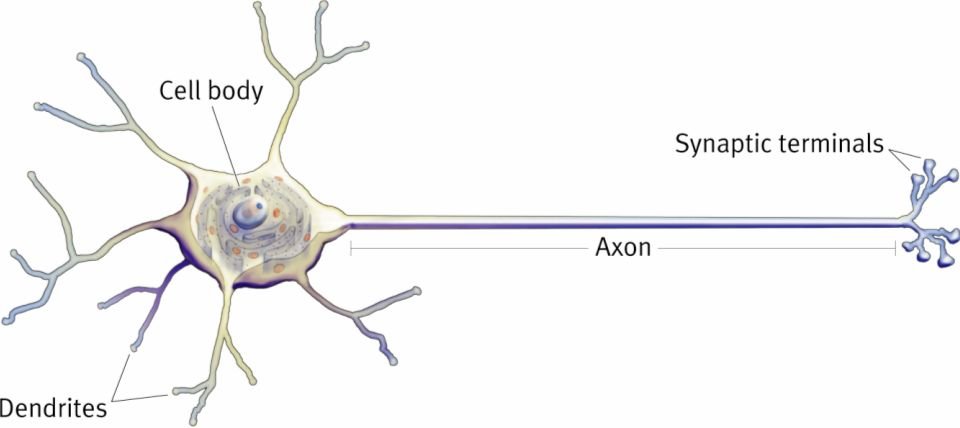
\includegraphics[width=0.8\textwidth,scale=1]{files/neuron.jpg}  
\caption{The parts of a nerve cell or neuron as shown in \cite{NEU}.}
\label{fig:neuron}
\end{figure}
\end{center}


Inspired by his hypothesis, some of the earliest work in the field of Artifical Intelligence aimed on building a similar srucure, a so called artifical neural network. \marginpar{\textit{The artifical neuron}}The general idea of this approach perceives the neuron as a basic Input/Ouput unit, which somehow processes the signals of other neurons and propagades its result further into the network. The funcion of the synpases is simply reproduced by altering each individual input by a  factor which is constantly modified by a certain percentage. This never-ending modificaion of all the input weights represents the learning effect of an artifical neuron. Figure \ref{fig:mathneuron} shows a simple mathematical model of a neuron which was first devised by \cite{NEURONMATH}. The artifical neurons output function is:\\

\begin{equation}
a_j = g(\sum_{i=0}^{} w_{i,j} \cdot a_{i})
\end{equation}

$a_{i}$ is the output of unit ${i}$ and $w_{i,j}$ the wight on the link from unit $i$ to unit $j$ (this unit). 


\begin{figure}[H]
\centering

\begin{tikzpicture}
\node [align=center] (in1) at (-0.5,0) {$a_i$}; 
\node [align=center] (in2) at (-0.3,0.75)   {}; 
\node [align=center] (in3) at (-0.8,1.5) {$a_i = 1$}; 
\node [align=center] (w1) at (0.7,0) {$w_{ij}$}; 
\node [align=center] (w3) at (0.7,1.5) {$w_{0j}$};
\node [align=center] (input) at (2,0.75) {\ \ $\sum_{}^{in_{j}}$}; 
\node [align=center] (function) at (4,0.75) {$\varphi$}; 
\node [align=center] (output) at (6,0.75) {$a_j$}; 
\node [align=center] (o1) at (8.5,0) {};
\node [align=center] (o2) at (8.5,0.75) {};
\node [align=center] (o3) at (8.5,1.5) {};

\node [align=center] (desilinks) at (0,-1) {Input\\ Links}; 
\node [align=center] (desinput) at (1.9,-1) {Input\\ funcion}; 
\node [align=center] (desfunc) at (4,-1) {Activation\\ function}; 
\node [align=center] (desoutput) at (6,-1) {Output}; 
\node [align=center] (desolinks) at (8,-1) {Output\\ links}; 

\node [align=center] (desweight) at (4,2) {$a_j = g(in_j)$}; 
\node [align=center] (desinfunc) at (0.75,2) {\small Bias Weight}; 
\node [align=center] (descneuron) at (6,1.5) {\small Cell body}; 

\node [align=center] (dummy1) at (2.4,0.75) {}; 
\node [align=center] (dummy2) at (5.36,0.75) {}; 

\draw[arrow]	(in1) -- (input);
\draw[arrow]	(in2) -- (input);
\draw[arrow]	(in3) -- (input);

\draw[arrow]	(output) -- (o1);
\draw[arrow]	(output) -- (o2);
\draw[arrow]	(output) -- (o3);

\node[draw=black,fit=(dummy1) (function) (dummy2) ,ellipse] (tmp) {};

\end{tikzpicture}
\caption{A mathematical model of a neuron}
\label{fig:mathneuron}
\end{figure}

\subsection{Units, Activity and Training}

The units in a representation of a neural network on a computer are divided into 3 classes, depending on their position in the network. \marginpar{\textit{Layers}}Neurons which reseve input from external sources, e.g. sensors, are called Input units and simply latch  their input into the next layer of neurons. At the other end of the network, the output layer which represents the last layer of the network, can be found. Its output is collected and evaluated by a logic that utilizes the neural network as a black box. In between those layers, a variable amount of so-called hidden layers can be found. They represent the networks \textbf{backbone so lassen?} or center. The complexity of the network increases by the amount of hidden layers. Figure \ref{fig:3layer} shows a three layer (sometimes called two layer, since the input layer does no computation) neural network. 
In order to allow computers quick and easy calculations, weights are often stored in matrices, representing the whole model as a basic mathematical unit. Let $N_{i}$ be a neural network, consisting of $i$ layers: Input,  output and $i-2$ hidden layers. $N_{i}$ can be fully described by $i-1$ matrices $W_{i,j}$ where $i$ is the number of units in the preceding layer, and $j$ the amount of neurons that are connected to any of those $i$ units:
\begin{equation}
W_{i,j} = 
\begin{pmatrix}
w_{1,1} & \cdots & w_{i,1} \\
\vdots & \ddots & \vdots \\
w_{1,j} & \cdots & w_{i,j} \\
\end{pmatrix}
\end{equation}





In addition, the concept of Bias Neurons has proven itself useful. Bias units  \marginpar{\textit{Bias-Units}} are neurons, which don't receive any input signals and have a fixed output of $+ 1$, although the weight on the connection link may be $\pm 1$. The Bias-Unit connected to a link with a positive weight is used to keep Neurons \textit{alive}, if they don't receive a significant input. On the contrary, a negative link may be used to keep a neuron in an inactive state.
Another application ist the implementation of a threshold value on a unit, preventing it from fireing too often.\\ 

As discussed before, the weights of the connections between the neurons represent the 'Intelligence' of the network. The bigger the absolute value of the weight, the greater the influence of a neuron to another. This value can be both positive and negative, as well as neutral \textit{(0)}, meaning that there is currently no influence between the neurons, although there is still a link connecting them. A weight of 0 can be understood as a logical pinch of the link, preventing it from transmitting signals.

\begin{figure}[H]
\centering

\begin{tikzpicture}
\node [draw=red, fill=red, align=center, circle] (i1) at (0,3) {}; 
\node [draw=red, fill=red, align=center, circle] (i2) at (0,2) {}; 
\node [draw=red, fill=red, align=center, circle] (i3) at (0,1) {}; 
\node [draw=red, fill=red, align=center, circle] (i4) at (0,0) {}; 

\node [draw=blue, fill=blue, align=center, circle] (h1) at (2,2.5) {}; 
\node [draw=blue, fill=blue, align=center, circle] (h2) at (2,1.5) {};
\node [draw=blue, fill=blue, align=center, circle] (h3) at (2,0.5) {};

\node [draw=green, fill=green, align=center, circle] (o1) at (4,2) {};
\node [draw=green, fill=green, align=center, circle] (o2) at (4,1) {};

\draw[arrow]	(i1) -- (h1);
\draw[arrow]	(i1) -- (h2);
\draw[arrow]	(i1) -- (h3);

\draw[arrow]	(i2) -- (h1);
\draw[arrow]	(i2) -- (h2);
\draw[arrow]	(i2) -- (h3);

\draw[arrow]	(i3) -- (h1);
\draw[arrow]	(i3) -- (h2);
\draw[arrow]	(i3) -- (h3);

\draw[arrow]	(i4) -- (h1);
\draw[arrow]	(i4) -- (h2);
\draw[arrow]	(i4) -- (h3);

\draw[arrow]	(h1) -- (o1);
\draw[arrow]	(h1) -- (o2);

\draw[arrow]	(h2) -- (o1);
\draw[arrow]	(h2) -- (o2);

\draw[arrow]	(h3) -- (o1);
\draw[arrow]	(h3) -- (o2);

\node[draw=red,fit=(i1) (i2) (i3) (i4),ellipse] (inputLayer) {};
\node[draw=blue,fit=(h1) (h2) (h3) ,ellipse] (hiddenLayer) {};
\node[draw=green,fit=(o1) (o2) ,ellipse] (outputLayer) {};

\node [align=center] (di) at (0,5) {\textcolor{red}Input\\ Layer};
\node [align=center] (dh) at (2,5) {\textcolor{blue}Hidden\\ Layer};
\node [align=center] (do) at (4,5) {\textcolor{green}Output\\ Layer};


\end{tikzpicture}
\caption{A three-layer neural network}
\label{fig:3layer}
\end{figure}

The connection between the input values and the activity level of the neuron is made by the activity function $\varphi$.\marginpar{\textit{Activity}} Different models are obtained depending on the choice of the activity or transfer function. Amongst the most common choices are the linear, binary step and sigmoid function as illustrated in Figure \ref{fig:plots}. The linear function has a threshold $t$, which can be used to avoid low network input (e.g. noise) to be further propagted into the network. The binary step function represents the firing of a pulse down the axon if positive $1$), while $0$ represents no firing. The step function is sometimes defined to jump from $-1$ to $1$. 

Sigmoid functions are widely used amongst network which are to represent cognitive processes such as perception, recoginition, problem solving, etc. .
Both the logistic function as well as the hyperbolic tangent function $\tanh()$ can be used. The main advantage of sigmoid functions are:

\begin{itemize}
\item In contrast with the linear function (without a threshold), the activity level of the function is limited in both the positive and the negative. This means that activity in the network can not spill over unintentionally, which can be caused by recurrent connections.
\item Differentiability
As distinct from the binary step function, it is differntiable at all parts, which as an example, is a requirement of the gradient descent, used by the Backpropagation algorithm (about to be introdced in section \ref{sec:learning}
\end{itemize}


\begin{figure}[H]
\centering
\subfigure[]
{
   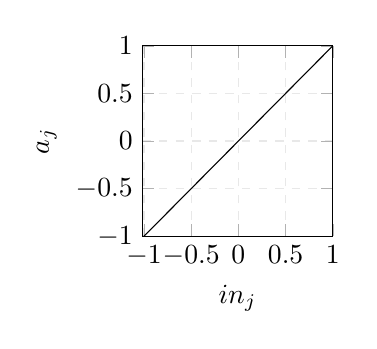
\begin{tikzpicture}
		\begin{axis}[
        width=4cm, height=4cm,     % size of the image
        grid = major,
        grid style={dashed, gray!30},
		xmax=1,        
        ymin=-1,
        ymax=1,
        axis background/.style={fill=white},
        ylabel=$a_{j}$,
        xlabel=$in_{j}$]
     
		\addplot[black]{x};
		\end{axis}
	\end{tikzpicture}
\label{fig:plot1}
}

\subfigure[]
{
   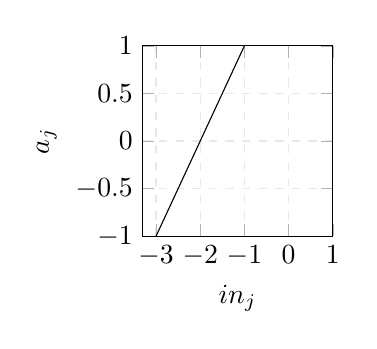
\begin{tikzpicture}
		\begin{axis}[
        width=4cm, height=4cm,     % size of the image
        grid = major,
        grid style={dashed, gray!30},
		xmax=1,        
        ymin=-1,
        ymax=1,
        axis background/.style={fill=white},
        ylabel=$a_{j}$,
        xlabel=$in_{j}$]
     
		\addplot[black]{x+2};
		\end{axis}
	\end{tikzpicture}
\label{fig:plot2}
}

\subfigure[]
{
   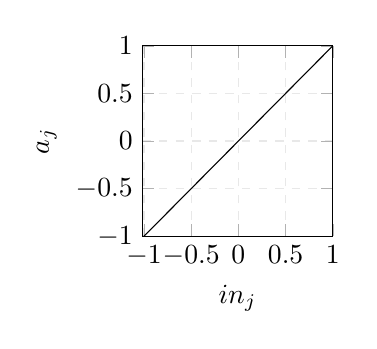
\begin{tikzpicture}
		\begin{axis}[
        width=4cm, height=4cm,     % size of the image
        grid = major,
        grid style={dashed, gray!30},
		xmax=1,        
        ymin=-1,
        ymax=1,
        axis background/.style={fill=white},
        ylabel=$a_{j}$,
        xlabel=$in_{j}$]
     
		\addplot[black]{x};
		\end{axis}
	\end{tikzpicture}
\label{fig:plot2}
}

	
\caption{Comparison of commonly used activation functions}
\label{fig:plots}
\end{figure}

In order to teach neural networks and enbale them to apply learned behavior in following scenarios, the work with them is divided in a training- and test phase. During the training, the network learns certain behavior by feeding repetitive input to the first layer and observing the output of the network. This can be done in a supervised and unsupervised way. In a supervised training phase, the targeted output of the network is already known and is presented to the network as a \textit{teaching factor}. The network produces output depending on the current weights on its connections and adjusts them acordingly to the margin between the targeted and produced output. Unsupervised learning is necessary in situations, where no reasonable teaching factors are available or the observant is more interested on the performance. Similarity between input incentives and connection weights is the factor, acording to which weight adjustment is done in such models.

\section{Learning}\label{sec:learning}
\subsection{Hebbian learning rule}
The psychologist Donald Olding Hebb proposed on the easiest learning rules with high biological plausibility in \cite{HEBB}:\\

\textit{``Let us assume that the persistence or repetition of a reverberatory activity (or "trace") tends to induce lasting cellular changes that add to its stability.… When an axon of cell A is near enough to excite a cell B and repeatedly or persistently takes part in firing it, some growth process or metabolic change takes place in one or both cells such that A's efficiency, as one of the cells firing B, is increased.''}\\

In summary: The weight between two units $i$ and $j$ is changed, if both units are active at the same time. The amount of change is set by three factors:

\begin{itemize}
\item The activity level of the sending unit $a_i$.
\item The activity level of the receiving unit $a_j$.
\item A settled and constant paramter $\eta$
\end{itemize}

The weight change $\Delta w_{ij}$ using the bian learning rule is shown in equation \eqref{eq:hebb}.
\begin{equation}
\Delta w_{i,j} = \eta \cdot a_i \cdot a_j
\label{eq:hebb}
\end{equation}

One of the major drawbacks of the hebbian rule is the fact, that is can only applied on networks without a hidden layer, and therefore only very simple neural networks.

\subsection{Delta rule}
The delta rule is based on the comparison between a targeted output $t$ and the observed output $o$ and can therefore only be applied with supervised learning.
It can be expressed using equation \eqref{eq:delta1}.
\begin{equation}
\delta = t - o
\label{eq:delta1}
\end{equation}

The following possibilities can be observed:
\begin{itemize}
\item \textbf{The observed output is too low}\\
In order to amplify the output, the weights between neurons is strengthened, provided a positive weight on the connection linking them. Negative weights are weakened.
\item \textbf{The observed output is too high}\\
All connections with positiv weights are weakened, while the ones with negative weights are strengthened 
\item \textbf{Targeted and observed output are equivalent. (= ideal behavior)}\\ There is no need to change the links.
\end{itemize}

The deltas learning rule equation \eqref{eq:delta2} covers all three posiblities, thus ensuring that the changing rate is proportional to the difference between targeted and observed. The learning paramter $\eta$ is again set before the beginning of the learning process and remains constant. The multiplication with the sending units output $a_i$ esures that those connections, that have the greatest influence into the error have the greatest $\delta w_{i,j}$.
\begin{equation}
\Delta w_{i,j} = \eta \cdot \delta \cdot a_i
\label{eq:delta2}
\end{equation}

The simplicity of this learning rules also comes at great cost: The comparison only allows us to adjust connections which connect to the rightmost layer in the network. This fact restricts the application of this method from networks with a hidden layer. 

\subsection{Backpropargation}

The backpropargation algorithm is yet another learning rule for supervised networks, but in comparison to the hebbian and delta rules, it can also be applied for networks with $n$ numbers of hidden layers. There are certain problems that cannot be solved by networks without at least one hidden layer, the XOR-Gate being an famous example for such problems. I was first  by Paul Werbos in 1975 \cite{BACK} and consists of three main steps:
\begin{itemize}
\item[1.] \textbf{The forward-pass}:
A pattern is presented to the input layer and further propargated into the network.
\item[2.] \textbf{Error-determination}:\\
The observed output is compared to targeted result and an error $E$ is determined by a derivale error-function $\varphi$ shown in equation \eqref{eq:backerror}. The factor of $\frac{1}{2}$ is used to simplify the derivation by cancelling the exponent.

\begin{equation}
\varphi = \frac{1}{2} (t-o)^2
\label{eq:backerror}
\end{equation}
\item[3.] \textbf{Backward-pass}:\\
The error is propargated from the back of the network to the front, hence the name \textbf{Backpropargation}. The connection are updated independent from their influence to $E$, which guarantees a result $o$ that is closer to $t$, provided the same output is presented to the input layer.
\end{itemize}

A first approach on finding a method to changing all weights in a weight that will minimize the error is to find $E$ for all possible combinations of weights $W$. The combination $W_{min}$ with the smallest $E$ would be the perfect solution, an abolute minimum of the error. The problem of this approach is that the computitional effort to finding this solution is way to high, since $W_{min}$ would have to be found in a $n$-dimensonial  hyperplane (given the number of neurons $n$).\\

Instead, the weights are adjusted using the gradient descent, which does not need to know the complete hyperplane\marginpar{\textit{gradient descent}}. It starts with a random combination of weights for which the gradient is determinded. The gradient is the function of a scalar field which shows the rate of change and the direction of the greatest change in the form of a vector field. After the gradient is determined it will be stepped down at a given rate - the learning rate, meaning that the weights are adjusted. For this new combination of weights, the gradient is again determined and stepped down until a local (or global minimum) is found or a maximum amount of repetitions is reached.\\

The amount of change between neurons $i$ and $j$ $\delta w_{i,j}$ is calculated as shown in \eqref{eq:backrule}.
\begin{equation}
\Delta w_{i,j} = -\eta \frac{\partial E}{\partial w_{i,j}} = \eta \cdot \delta_j \cdot a_i
\label{eq:backrule}
\end{equation}
As distinct form the delta rule, the backpropargation rule differs two cases, shown in equation \eqref{eq:backcases}. $k$ is the index of the neurons in the subsequent layer.
\begin{equation}
   \delta_j =
   \begin{cases}
     \varphi'(in_j)(t_j-o_j) & \text{In case j is an output neuron} \\
     \varphi'(in_j)\sum_{k} \delta_k \cdot w_{j,k} & \text{In case j is a hidden neuron}
   \end{cases}
\label{eq:backcases}
\end{equation}

Eventuall the weights are changed acording to equation \eqref{eq:backweight}.

\begin{equation}
   w_{i,j}^{new} = w_{i,j}^{old} + \Delta w_{i,j}
\label{eq:backweight}
\end{equation}

\subsection{Backpropargation through time}
\subsection{Competitive learning}
%...
\section{Network types}
At the moment there are three generations of neural networks. 
The first generation works with binary in- and outputs, but real thresholds. The first model was presented in 1943.
In the second generation, presented in the 90s, the firerates symbolizes real values transmitted on in- and outputs. Real thresholds are still used.
The newest generation uses spikes, an encoding through time.

\subsection{First generation}
The first generation of neural networks have binary in- and outputs.

\subsubsection{McCulloch-Pitts neuron}
The first mathematical model of a neuron was the McCulloch-Pitts-neuron,
developed by Warren McCulloch and Walter Pitts in 1943.
They wanted to realise a simple, realistic neuron-modell of operations in the brain and find out if the brain could compute turing computability functions.
McCulloch-Pitts-neuron has binary in- and outputs.
A real threshold can be defined, which reached, let the neuron fire an one, otherwise zero.
Its possible to add absolute suppressing inputs. If one of these has the value one, the neuron gives out zero, no matter of other inputs. The use of such absolute supressing inputs is for the most cases doubtfull.


Neural networks of this type of neuron can just learn by changing topology of the network, that is laborious.

At the following a figure of a single neuron:

\begin{figure}[H]  % [H] erzwingt Position an der Stelle im Text
	\centering
	\begin{tikzpicture}
	\node [align=center] (dummy1) at (-0.25,3.5) {$x_{1}$}; 
	\node [align=center] (dummy2) at (-0.25,2.5) {$x_{n}$}; 
	\node [draw=black, fill=white, align=center, circle] (f1) at (1,3) {f}; 		
	\node [align=center] (dummy3) at (3,3) {f($x_{1}$,..,$x_{n}$)}; 
	\draw[arrow]	(dummy1) -- (f1);
	\draw[arrow]	(dummy2) -- (f1);
	\draw[arrow]	(f1) -- (dummy3);
	\draw[dotted] (dummy1) -- (dummy2);
	
	\end{tikzpicture}
	\caption{A McCulloch-Pitts-neuron}
	\label{fig:pitts1}
\end{figure}
The neuroninput is computed by:

\begin{equation}
	neuroninput = \sum_{i=1}^{n} x_{n} \quad  x \in \{0, 1\}
\end{equation}

The output is given by:

\begin{equation}
	neuronoutput=\begin{cases}
		0 \quad  neuroninput < S \\  % Or minimum 1 supressing input is 1
		1 \quad  neuroninput \geq S \\
	\end{cases}
	S \in \mathbb{R}
\end{equation}

A function composition:

\begin{figure}[H]
	\centering
	\begin{tikzpicture}
	\node [align=center] (dummy1) at (-0.25,3.5) {$x_{1}$}; 
	\node [align=center] (dummy2) at (-0.25,2.5) {$x_{n}$}; 
	\node [draw=black, fill=white, align=center, circle] (f1) at (1,3) {f}; 		
	\node [draw=black, fill=white, align=center, circle] (g1) at (2.5,3) {g}; 
	\node [align=center] (dummy3) at (4.5,3) {f(g($x_{1}$,..,$x_{n}$)}; 
	\draw[arrow]	(dummy1) -- (f1);
	\draw[arrow]	(dummy2) -- (f1);
	\draw[arrow]	(f1) -- (g1);
	\draw[arrow]	(g1) -- (dummy3);
	\draw[dotted] (dummy1) -- (dummy2);
	
	\end{tikzpicture}
	\caption{Function composition of two McCulloch-Pitts-neurons}
	\label{fig:pitts2}
\end{figure}

A recursive neuron:

\begin{figure}[H]
	\centering
	\begin{tikzpicture}
	\node [align=center] (dummy1) at (-0.25,3) {$x_{t}$}; 
	\node [draw=black, fill=white, align=center, circle] (f1) at (1,3) {f}; 		
	\node [align=center] (dummy2) at (4,3) {f($x_{t}$,f($x_{t-1}$,f($x_{t-2}$,...)))}; 
	\draw[arrow]	(dummy1) -- (f1);
	\draw[arrow]	(f1) -- (dummy2);
	\draw[arrow]	(f1) -- (f1);
	\draw[->] (1.35,3) .. controls (1.3,2.15) and (0.6,2.2) .. (0.65, 3);
	\end{tikzpicture}
	\caption{Recursive McCulloch-Pitts-neuron}
	\label{fig:pitts3}
\end{figure}

The output is given after a fixed timestep t.

\paragraph{Applications}
The McCulloch-Pitts-neuron is biologically not plausible, because learning
can just happen by changing the threshold and the network topology. This
needs complex algorithms.
But this neuron type can realise AND-, OR- and NOT-Gates.
Therefore a network of neurons can realise every boolean logic and it is used in electrical engineering, because of realising logic gates efficently in contrast to classical gates. You can simulate finite state machines, too.
You may think if its better to have real or at least integer values to transmit more information instead of just binary signals. This depends on the applicationtype. Binary values are easier to realize, both in electrical and biological systems and mcculloch-pitts-networks are equivalent to other kind of networks with more signalstates. Though you get a more complex networktopology, if you use binary neurons.

It was the first mathematical model of artifical neural networks.\cite{NEURONMATH}


\subsubsection{Perceptron}
The classical perceptron was published by Frank Rosenblatt in 1958.
It has an input- and an outputlayer with binary values. In contrast to the McCulloch-Pitts-neuron
the perceptron has real weights. The advantage is that learning-algorithms has just to change the weights
instead of the topology. Its possible to define positive (stimulation), negative (supression) and zero(neutral) weights.

\paragraph{Linear seperability}
A classical perceptron can only seperate linear datasets. This is due to only two layers. For seperating non-linear datasets read \ref{sec:mlp}.
An widely known example is the xor-problem.

\begin{figure}[H]
	\centering
%	\subfigure[]
%	{
\begin{tabular}{|l|l|l|}
	\hline
	x1 & x2 & f6\\
	\hline
	0 & 0 & 0 \\
	\hline
	0 & 1 & 1 \\
	\hline
	1 & 0 & 1 \\
	\hline
	1 & 1 & 0 \\
	\hline
\end{tabular}
%}
	\caption{XOR-Function: Not linear seperable}
	\label{fig:linsep1}
	
		\subfigure[]
		{
			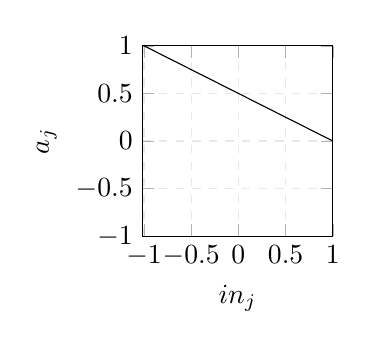
\begin{tikzpicture}
			\begin{axis}[
			width=4cm, height=4cm,     % size of the image
			grid = major,
			grid style={dashed, gray!30},
			xmax=1,        
			ymin=-1,
			ymax=1,
			axis background/.style={fill=white},
			ylabel=$a_{j}$,
			xlabel=$in_{j}$]
			
			\addplot[black]{-0.5*x+0.5};
		%	\addplot[black]{-2*x-1.5};
			\end{axis}
			\end{tikzpicture}
			\label{fig:sepplot1}
		}
		
\end{figure}

\paragraph{Applications}
The perceptron can be used as pattern associator to categorise an inputpattern to a class, competitive network. Also linear seperable data can be categorised.
It can be trained with the hebbian- or the delta-learning rule.(see also \eqref{sec:learning})

\begin{center}
	\begin{figure}[H]
		\centering
		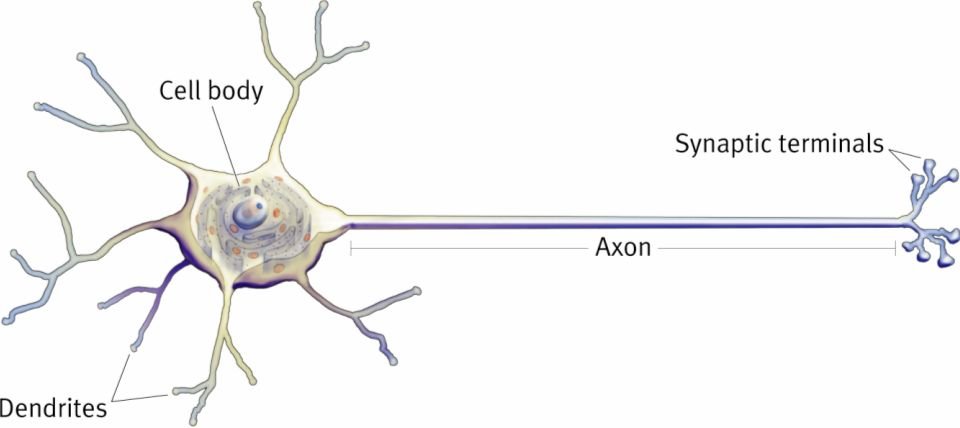
\includegraphics[width=0.8\textwidth,scale=1]{files/neuron.jpg}  
		\caption{A singlelayer perceptron \cite{PERSIN}.}
		\label{fig:neuron}
	\end{figure}
\end{center}

\subsection{Second generation}
The idea of the second generation of neural networks is born in the 90s. The firerate of a neuron encodes the transmitted signal. In this case now real values are used for in- and outputs.

\subsubsection{Multi layer perceptron (MLP)} \label{sec:mlp}
The multilayer perceptron was intruduced by Minsky and Papert in . It has an input-, an output- and
one or multiple hiddenlayers. In contrast to the singlelayerperceptron it can solve the xor-problem and other non-linear problems. It can be trained super- or unsupervised.

\paragraph{Applications}

\subsubsection{Radial basis function} %Oder paragraph?


\subsubsection{Kohonen networks / Selforganizing maps (SOM)}
Kohonen-networks are inventioned by the finnish engineer Teuvo Kohonen in 1982. They have two layers. An inputlayer and a n-dimensional outputlayer.
Kohonen-networks usually don't have hidden layers.
The inputspace 

\paragraph{Applications}
Data-mining, unsupervised learning, clusteranalysis, computergraphics. 

\subsection{Combination of networkmodels}

\subsubsection{MLP and SOM} %look at neuronale netze im klartext chapter 6.3

\subsection{Third generation}
In the third generation of artifical neural networks the signal is additionally encoded in time. These called spikes are

\subsubsection{Spiking neural networks}

\paragraph{Applications}

%\subsection{Feed Forward}
\subsection{Recurrent}

\paragraph{Applications}

%...
%\section{Applications}
%\subsection{Pattern recognition}

%\subsection{Traveling salesman problem}

%\subsection{Aproximation of functions}
%...

\chapter{Optimization with evolutionary algorithms}
Optimization is widely used, for example in information technology, engineering,
economics, etc. Applications are the routing of circuits, the optimal usage of machinery,
the traveling-salesman-problem and much more. It is often difficult to create a mathematical
model of such optimization problems. Therefore in the last decades were developed methods who
uses principles of the evolution.
The simples method is the selection-method. In this model a dateset will be generated and randomly
changes, called mutations, are made. The best datasets, chosen by the best fitness, will be kept.
Each dateset is called an individual. A set of individuals is called a population. The individuals
of a population can be recombined. Mostly the best individuals are recombined with randomly chosen
ones. This method is more effective than the selection-method. This and other methods are  called
evolutionary algorithms. To use an evolutionary algorithm, the problem must not be in a defined form;
therefore it hasn't to be linear or differentiable. \\

In this project evolutionary algortihms are used to find the best 
(unsupervised) neural network to controll one creature. The idea is to use the amount of food a creature collect over a defined time as fitnessvalue.

\section{The creepy random search method or hill climber method}
The creepy random search method is a basic method of an evolutionary algorithm, developed by Ingo Rechenberg in 1973. % 1973 correct?? look at literaturesource in kinnebruck
Parameters of a system are randomly changed till a minimum or maximum of a targetfunction is reached. The value of the parameterchanges per iterationstep are limited. \\

\textbf{The main algorithm is:}

\fbox{
\begin{minipage}{15cm}
	\begin{enumerate} 
		\item Generate a randomly initialized chromosome.
		\item Change the chromosome parameter by limited random delta-values. 
		\item Prove if the chromosome has a better fitness than the old one and replace it. Otherwise forget the new chromosome.
		\item If the optimization-condition is reached abort, otherwise go to step 2.
	\end{enumerate}
\end{minipage}
} \\

The algorihm can be imagined as a blind hillclimber. The hillclimber makes a random step. If he gets higher, he makes the next step. Otherwise he takes back his last step and makes another random step. The big problem is, that this algorithm mostly converges in a local optimum. \\

\textbf{Reasons to use this kind of algorithm:}

\fbox{
	\begin{minipage}{15cm}
		\begin{itemize} 
			\item For many nonlinear problems there are no alternative solution approaches.
			\item Implementing this method is easy.
		\end{itemize}
	\end{minipage}
}   \\



\begin{center}
	\begin{figure}[H]
		\centering
		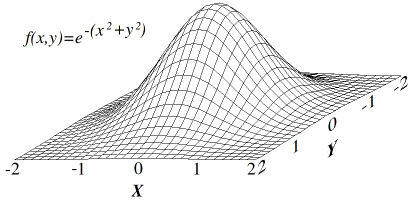
\includegraphics[width=0.6\textwidth,scale=1]{files/Hill_climb.png}  
		\caption{A convex function. Ideal for the hillclimbing method \cite{wiki-hill}.}
		\label{fig:hill}
	\end{figure}
\end{center}

\begin{center}
	\begin{figure}[H]
		\centering
		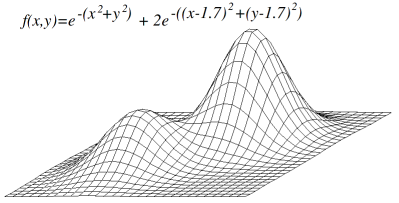
\includegraphics[width=0.6\textwidth,scale=1]{files/Local_maximum.png}  
		\caption{A function with two optima. Hillclimbing could end in the worse optimum if it starts at a bad coordinate. \cite{wiki-hill}.}
		\label{fig:hill2}
	\end{figure}
\end{center}


\subsection{Constraints} %Bedingungen und Nebenbedingungen
The main condition is the fitness-function. Second conditions
can be the

%\subsection{Efficency} %Optional chapter to test the efficency between mathematical methods and evolutionary methods. For example zero of a function.

\section{Variants of the creepy random search method}
In the main-method of the creepy random search you just accept better fitness values after an iteration-step and reject worse ones.
The problem is, that with this algorithm you will mostly get stuck on a local optimum, instead of finding the global one.
To solve this problem you should allow temporal low fitness-values. It should be possible to leave a local optimum to find a better one.
To realise this, there have been developed some extended versions of this method: \\

\fbox{
	\begin{minipage}{15cm}
		\begin{itemize} 
			\item A stagnation of the fitness is allowed by a specified probability (Simulated annealing)
			\item A stagnation of the fitness is allowed till a maximal deterioration. (Threshold accepting, deluge method)
		\end{itemize}
	\end{minipage}
} \\


\subsection{Simulated annealing}
Simulated annealing is a probabilistic optimization method.
It is inspired by the annealing of fluid materia to a solid aggregate states in metallurgy. While cooling down a material the thermodynamic free energy has to get as minimal as possible to get a clear crystalline structure. Therefore its suggested to cool down to material slowly for a better probability of getting a clear solid body.

Analog in optimization you start with a high temperature T, means a big delta, to make wide jumps in the problemphase-space. So jumps between more maxima are possible. At the beginning each chromosome has the same probability to get selected. With each iteration the temperature is reduced and the jumps are getting shorter. Selecting better chromosomes is now more probalistic.
Towards the end the algorithm commutes in a optimum and behaves like the standard hillclimbing-algorithm.

Slowly reducing the temperature increases the chance to find the global optimum. Cooling to fast leads to commuting early into a local optimum instead.

The following formula shows the probability of selecting a chromosome with lower fitness:

\begin{equation}
p(r) = \frac{1}{1+exp(-r/T)}
\end{equation} 

The probability to select a worse chromosome should be small.
At the beginning a big T tends to equalize the probability of all chromosomes. For $T \to \infty$ all chromosomes have the same chance to get selected. Lowering T gives good chromosomes priority. For T = 0.1

\subsection{Threshold accepting}

\section{Genetic algorithms - An artifical duck}

\section{}

\chapter{Other 'intelligent' algorithms}
In this chapter other intelligent algorithms are presented.
These algortihms are for comparing the neural network to simpler
methods.

\section{The greedy algorithm}

\subsection{Weaknesses}



\KOMAoptions{listof=leveldown}

\newpage

%=========================================LISTS=========================================

\listoffigures
\listoftables
\listofalgorithms
\lstlistoflistings

\newpage

%=========================================DICTIONARY====================================

%dictiary style
\bibliographystyle{./files/alphadin}
%dictionary source
\bibliography{./files/bibdb}

\end{document}
